% =====================================================================
%  Climate Solutions and Strategies | Assignment 1
%  Policy memo: Why limiting climate change matters for Niger
%  Author: KOUAME Koffi Fidele, IMP-EGH, Abdou Moumouni University
%  Compile: pdflatex niger_policy_memo.tex (twice)
% =====================================================================
\documentclass[10pt,a4paper]{article}

% Cover page on (true) or off (false). The memo itself is 2 pages either way;
% references are on the following page.
\newif\ifcover
\covertrue

\usepackage[T1]{fontenc}
\usepackage[utf8]{inputenc}
\usepackage{tgtermes}
\usepackage{mathptmx}
\usepackage[english]{babel}
\usepackage[a4paper,top=1.9cm,bottom=1.7cm,left=1.9cm,right=1.9cm,headsep=0.5cm,footskip=0.8cm]{geometry}
\usepackage{microtype}
\usepackage{amsmath,amssymb}
\usepackage{xcolor}
\usepackage{graphicx}
\usepackage{tabularx,array,booktabs}
\usepackage{enumitem}
\usepackage{titlesec}
\usepackage{fancyhdr}
\usepackage[most]{tcolorbox}
\usepackage[hidelinks]{hyperref}
\usepackage{xurl}
\usepackage{caption}
\usepackage{float}
\urlstyle{same}

% ---- colours (same palette as the IMP-EGH documents)
\definecolor{uamred}{HTML}{C00000}
\definecolor{egh}{HTML}{6AA84F}
\definecolor{rulegray}{HTML}{A59F93}
\definecolor{boxgray}{HTML}{E6E6E6}

% ---- layout
\setlength{\parindent}{0pt}
\setlength{\parskip}{3pt}
\setlist{nosep,itemsep=1.5pt,leftmargin=1.3em}
\captionsetup{font=small,labelfont=bf,skip=3pt}

\titleformat{\section}{\large\bfseries}{}{0pt}{}
\titlespacing*{\section}{0pt}{8pt}{3pt}

\pagestyle{fancy}
\fancyhf{}
\fancyhead[L]{\small\textbf{Climate Solutions and Strategies | Policy memo}}
\fancyhead[R]{\small IMP-EGH | System Analysis | 2026}
\fancyfoot[C]{\small\thepage}
\renewcommand{\headrulewidth}{0.6pt}

\newcommand{\degC}{\,\textdegree C}
\newcommand{\rng}[1]{{\footnotesize [#1]}}
\newcolumntype{Y}{>{\raggedright\arraybackslash}X}
\newcolumntype{L}[1]{>{\raggedright\arraybackslash}p{#1}}
\newcolumntype{C}[1]{>{\centering\arraybackslash}p{#1}}

% gray box with black left rule, as the "Instructions" box of the IMP-EGH sheets
\newtcolorbox{graybox}[1]{colback=boxgray!35,colframe=black,boxrule=0pt,leftrule=2.5pt,arc=0pt,
  left=6pt,right=6pt,top=2pt,bottom=3pt,
  title={\textbf{#1}},coltitle=black,colbacktitle=boxgray,attach title to upper={\par\smallskip}}

\begin{document}

% =====================================================================
%  COVER PAGE
% =====================================================================
\ifcover
\begin{titlepage}
\thispagestyle{empty}
\begin{minipage}[c]{0.2\textwidth}
  
\includegraphics[width=\linewidth]{logo_uam.png}
\end{minipage}%
\begin{minipage}[c]{0.58\textwidth}
  \centering
  {\Large\bfseries\textcolor{uamred}{A}bdou \textcolor{uamred}{M}oumouni \textcolor{uamred}{U}niversity}\\[6pt]
  {\small\bfseries\textcolor{egh}{I}nternational \textcolor{egh}{M}aster \textcolor{egh}{P}rogram in
   \textcolor{egh}{E}nergy and \textcolor{egh}{G}reen \textcolor{egh}{H}ydrogen}\\[4pt]
  {\bfseries (IMP-EGH)}
\end{minipage}%
\begin{minipage}[c]{0.22\textwidth}
  \raggedleft
\includegraphics[width=0.95\linewidth]{logo_impegh.png}
\end{minipage}

\vspace{10pt}
{\color{rulegray}\rule{\textwidth}{2.2pt}}

\vspace*{4.6cm}
\begin{center}
{\fontsize{26}{32}\selectfont\bfseries Why Limiting Climate Change}\\[6pt]
{\fontsize{26}{32}\selectfont\bfseries Matters for Niger}\\[14pt]
{\Large\itshape Policy memo to the Government of Niger}\\[8pt]
{\large Climate Solutions and Strategies\quad Assignment 1\quad Country case study: Niger}\\[24pt]
{\large Assessing national climate risks with the Climate Impact Explorer}\\[2pt]
{\large and the national interest of limiting global warming}
\end{center}

\vfill
\begin{minipage}[t]{0.5\textwidth}
\textbf{Course}\\[3pt]
Climate Solutions and Strategies\\
Assignment 1, due 14 October 2026
\end{minipage}%
\begin{minipage}[t]{0.5\textwidth}
\raggedleft
\textbf{Prepared by}\\[3pt]
KOUAME Koffi Fidèle\\
IMP-EGH, option System Analysis
\end{minipage}

\vspace{2.2cm}
\begin{center}\textbf{October 2026}\end{center}
\end{titlepage}
\setcounter{page}{1}
\fi

% =====================================================================
%  MEMO, PAGE 1
% =====================================================================
\begin{center}
{\LARGE\bfseries Policy Memo | Why Limiting Climate Change Matters for Niger}\\[2pt]
{\large Advice to the national delegation to the UNFCCC}
\end{center}
\vspace{-4pt}

{\small
\renewcommand{\arraystretch}{1.35}
\begin{tabularx}{\linewidth}{|>{\raggedright\arraybackslash}X|>{\raggedright\arraybackslash}X|}
\hline
\textbf{To:} Minister of Environment, Head of Niger's UNFCCC delegation &
\textbf{From:} KOUAME Koffi Fidèle, Climate Adviser \\
\hline
\textbf{Date:} 14 October 2026 &
\textbf{Subject:} What Niger stands to lose, and to gain if warming is limited \\
\hline
\end{tabularx}}

\vspace{4pt}
\begin{graybox}{Key message}
\textbf{Under current global policies, Niger would face about 91 days a year of dangerous heat by 2100, three
times today's 31; if the world holds warming below 2\degC, that number stabilises at around 42.} In an
economy where farming and herding employ more than 80\,\% of people, mostly outdoors, this is the largest
avoidable loss. Current policies would also make the heaviest multi-day rains about 43\,\% more intense,
against 17\,\% below 2\degC. Severe drought months, however, will touch almost the whole country by 2030 in
every scenario, so \textbf{Niger must both push for a rapid global phase-out of emissions and invest in
adaptation now.}
\end{graybox}

\section{1. Why Niger is unusually exposed, and not responsible}
\begin{itemize}
  \item \textbf{An open-air economy.} Agriculture and livestock account for almost 40\,\% of GDP and over
        80\,\% of jobs, and depend overwhelmingly on rainfall (World Bank, 2024).
  \item \textbf{Shocks are already frequent and costly.} The 2005 and 2010 droughts triggered national food
        crises; the 2024 floods killed 339 people and affected more than 1.1 million (AFP, 2024).
  \item \textbf{A negligible contributor.} Niger emits a tiny share of global greenhouse gases: the losses
        below are driven by others' emissions, and can only be limited by others' cuts.
\end{itemize}

\section{2. Three priority impacts: below 2\degC{} versus current policies}
{\small\itshape Source: Climate Impact Explorer (CIE), Niger, annual, area-weighted average. NGFS ``Below
2\degC'' (1.6\degC{} of global warming in 2100) versus ``Current policies'' (2.9\degC). Median of five
climate models, 5--95\,\% range in brackets; the CIE flags results after 2060 as indicative.\par}
\vspace{3pt}

{\small
\renewcommand{\arraystretch}{1.2}
\begin{tabularx}{\linewidth}{@{}L{2.75cm} C{1.45cm} C{2.15cm} C{2.15cm} Y@{}}
\toprule
\textbf{Impact (CIE indicator)} & \textbf{Today (2020)} & \textbf{Below 2\degC} &
\textbf{Current policies} & \textbf{Why it matters for Niger}\\
\midrule
\textbf{1. Dangerous heat}\newline{\footnotesize\itshape Days per year with heat index above 40\degC} &
\textbf{31 days}\newline\rng{25--38} &
2050: \textbf{45}\newline\rng{33--69}\par\vspace{2pt}2100: \textbf{42}\newline\rng{29--72} &
2050: \textbf{54}\newline\rng{41--84}\par\vspace{2pt}2100: \textbf{91}\newline\rng{59--134} &
Above this threshold, sustained outdoor work risks heat exhaustion and heat stroke, and most Nigeriens
farm, herd or build outdoors without cooling. CIE maps show a rise about twice as large in the populated
south as in the north (+44 versus +21 days at 2\degC{} compared with 1\degC{} of global warming). WASCAL
researchers project heat discomfort for over half of West Africa's population even at 1.5--2\degC{}
(Sylla et al., 2018). \\
\midrule
\textbf{2. Severe drought}\newline{\footnotesize\itshape Share of land with at least one month of SPEI
below $-1.5$ (\%)} &
\textbf{84\,\%}\newline\rng{72--97} &
2050: \textbf{98\,\%}\newline\rng{85--100}\par\vspace{2pt}2100: \textbf{98\,\%}\newline\rng{81--100} &
2050: \textbf{$\approx$100\,\%}\newline\rng{96--100}\par\vspace{2pt}2100: \textbf{100\,\%}\newline\rng{98--100} &
SPEI counts evaporation as well as rain, so it captures what heat does to soils, crops and pastures. By
2030, about 96\,\% of the country is affected in every scenario: severe drought months become the norm
whatever the world does. Only a 1.5\degC{} pathway brings this back down (87\,\% by 2100). WASCAL crop
modelling projects falling millet yields in most scenarios (Mohamed et al., 2025). \\
\midrule
\textbf{3. Extreme rainfall}\newline{\footnotesize\itshape Annual maximum 5-day precipitation, change from
1995--2014 (\%)} &
\textbf{+8\,\%}\newline\rng{$-$7 to +29} &
2050: \textbf{+18\,\%}\newline\rng{0 to +55}\par\vspace{2pt}2100: \textbf{+17\,\%}\newline\rng{$-$1 to +54} &
2050: \textbf{+24\,\%}\newline\rng{$-$1 to +67}\par\vspace{2pt}2100: \textbf{+43\,\%}\newline\rng{+5 to +110} &
Heavier downpours on bare, crusted soils flood Niamey and the Niger River valley, where people,
infrastructure and irrigated rice are concentrated. Under current policies, even the low end of the model
range shows an increase by 2100. Extreme Sahelian storms have already tripled in frequency since 1982
(Taylor et al., 2017). \\
\bottomrule
\end{tabularx}}

% =====================================================================
%  MEMO, PAGE 2
% =====================================================================
\begin{figure}[H]
\centering
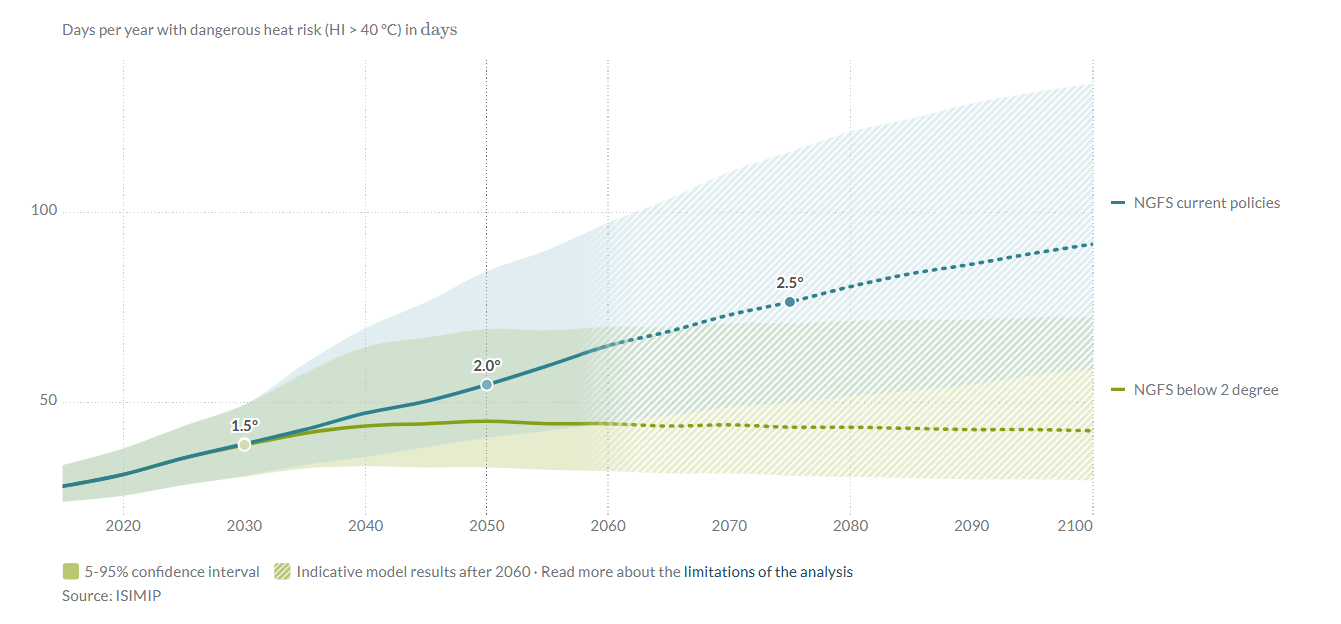
\includegraphics[width=\linewidth,height=7.6cm,keepaspectratio]{cie_figure.png}
\caption*{\small\textbf{Figure 1. Days of dangerous heat per year in Niger: the gap between the two curves is
what limiting warming saves.} The two paths are identical until about 2030, then diverge: by 2100, current
policies (blue) lead to about 91 days a year, against 42 below 2\degC{} (green) and 31 today. The shaded bands
(model uncertainty) overlap, but even the low end of the current-policies range (59 days) exceeds the central
below-2\degC{} estimate. Hatched area: results after 2060 are indicative. Source: Climate Impact Explorer,
Climate Analytics (ISIMIP data).}
\end{figure}
\vspace{-8pt}

\section{3. Implications for Niger's national interest}

\textbf{Heat is the largest avoidable loss.} Moving from current policies to a below-2\degC{} world avoids
roughly 50 days of dangerous heat a year by 2100, nearly two months in which outdoor work, livestock and
health are at risk. The World Bank (2022) estimates that climate change could cut Niger's annual GDP by
2.2\,\% (wet, optimistic scenario) to 11.9\,\% (dry, pessimistic scenario) by 2050, before counting migration
or conflict.

\textbf{Drought makes adaptation unavoidable in every scenario.} Since severe drought months spread to almost
the whole country by 2030 regardless of emissions, Niger cannot wait: drought-tolerant millet and sorghum,
water harvesting, early warning and protection of herders' mobility are needed now. The risk is a cascade:
hot, dry year $\rightarrow$ failed harvests and pastures $\rightarrow$ higher grain prices and distress sales
of livestock $\rightarrow$ malnutrition, debt and farmer--herder tensions $\rightarrow$ emergency spending that
crowds out investment.

\textbf{Floods grow with every tenth of a degree.} Extreme rainfall keeps intensifying under current policies
(+43\,\% by 2100) but levels off below 2\degC{} (+17\,\%). Limiting warming directly reduces the flood risk
facing Niamey and the river valley.

\begin{graybox}{Recommended negotiating position}
\begin{enumerate}[label=(\roman*)]
  \item Defend the 1.5\degC{} goal: it is the only pathway that brings heat days back to today's level
        (32 by 2100) and reverses drought spread; press major emitters for NDCs consistent with a rapid
        fossil-fuel phase-out.
  \item Tie Niger's support to scaled-up, accessible adaptation finance for Least Developed Countries.
  \item Use the Loss and Damage Fund for droughts and floods, in coalition with the African Group and the
        LDC group.
\end{enumerate}
\end{graybox}

\section{4. What the evidence does, and does not, say}
The direction of change is robust for heat; the size is not: by 2100 under current policies, models span 59
to 134 dangerous-heat days. Heat-index values rely on an approximation of humidity during the hottest hour, a
limitation the tool itself notes. The drought indicator counts a single month of severe drought, so it
saturates and barely separates scenarios. For extreme rainfall, the ranges include no change under low warming
but not under current policies by 2100. The tool's only crop indicators (maize, rice, soy) were set aside
because Niger's staples, millet and sorghum, are not modelled. Finally, these are hazard projections, not
forecasts; Niger's high social vulnerability means real impacts are likely to be larger.

% =====================================================================
%  REFERENCES (outside the 2-page limit)
% =====================================================================
\clearpage
\section{References}
{\small
\begin{list}{}{\leftmargin=1.4em \itemindent=-1.4em \itemsep=5pt \parsep=0pt}
\item AFP (2024, 9 October). Niger ups flood toll to 339 dead, more than 1 million affected.
      \emph{Inquirer.net}.
      \url{https://globalnation.inquirer.net/251812/niger-ups-flood-toll-to-339-dead-more-than-1-million-affected}
\item Climate Analytics (2026). \emph{Climate Impact Explorer}: Niger. Indicators: days per year with
      dangerous heat risk (HI $>$ 40\degC), area under severe drought (SPEI $< -1.5$), annual maximum 5-day
      precipitation; NGFS Below 2\degC, Current Policies and Net Zero 2050 scenarios; ISIMIP data.
      \url{https://climate-impact-explorer.climateanalytics.org} (accessed 9 October 2026).
\item Mohamed, A. M. L., Salack, S., Mkuhlani, S., Chemura, A., et al. (2025). Impact of climate change on
      millet yield under different fertilization levels in three agroecological zones of Niger Republic.
      \emph{PLOS ONE}, 20(10), e0333963. \url{https://doi.org/10.1371/journal.pone.0333963}
\item Sylla, M. B., Faye, A., Giorgi, F., Diedhiou, A., \& Kunstmann, H. (2018). Projected heat stress under
      1.5\degC{} and 2\degC{} global warming scenarios creates unprecedented discomfort for humans in West
      Africa. \emph{Earth's Future}, 6(7), 1029--1044. \url{https://doi.org/10.1029/2018EF000873}
\item Taylor, C. M., Belu\v{s}i\'{c}, D., Guichard, F., Parker, D. J., Vischel, T., Bock, O., Harris, P. P.,
      Janicot, S., Klein, C., \& Panthou, G. (2017). Frequency of extreme Sahelian storms tripled since 1982 in
      satellite observations. \emph{Nature}, 544, 475--478. \url{https://doi.org/10.1038/nature22069}
\item World Bank (2022). \emph{G5 Sahel Region Country Climate and Development Report}. CCDR Series.
      Washington, DC: World Bank. \url{http://hdl.handle.net/10986/37620}
\item World Bank (2024, 28 June). The World Bank supports food security and climate resilience for households
      in Niger [Press release].
      \url{https://www.worldbank.org/en/news/press-release/2024/07/01/the-world-bank-supports-food-security-and-climate-resilience-for-households-in-niger}
\end{list}}

\end{document}
